%%%%%%%%%%%%%%%%%%%%%%%%%%%%%%%%%%%%%%%%%
%% Results section
\section{Results}
\label{sec:results}

SUMMARY PARAGRAPH HERE.


\subsection{University-Level}

\autoref{tab:facultycount-shock-reg} presents OLS and IV estimates, where the outcome is (log) count of professors employed at the university, separated by position, and for all professors (Columns 7, 8).
For all professors we see a positive correlation between university revenues and professor count per student (the OLS columns), where an increase in university total revenues by 10\% is associated with an increase in professor count per student of 0.83\%, yet negatively correlated with lecturer count of -1.3\%.
Lecturers per student is not shown to be correlated with total university revenues.
The 2SLS columns show results after identifying state funding with the appropriation shock.
All professor count per student increases by 0.53\% in response to a 10\% rise in total revenues.
The effect is driven by increases in the count of assistant and full professors (i.e. tenure-track and tenured) per student, where assistant professor count per student increase by 1.4\%, and full professor 1.2\%.
The count of lecturers per student decreases by 4.4\% in response to a (positive) 10\% shock in university revenues.

\begin{table}[h!]
    \singlespacing
    \centering
    \caption{OLS and 2SLS Estimates for University Faculty Composition.}
    \makebox[\textwidth][c]{
\begin{tabular}{@{\extracolsep{5pt}}lcccccccc} 
\\[-1.8ex]\hline 
\hline \\[-1.8ex] 
 & \multicolumn{8}{c}{Dependent Variable: Employment Count by Professor Group} \\ 
\cline{2-9} 
\\[-1.8ex] & \multicolumn{2}{c}{Lecturer} & \multicolumn{2}{c}{Assistant} & \multicolumn{2}{c}{Full} & \multicolumn{2}{c}{All} \\ 
 & OLS & 2SLS & OLS & 2SLS & OLS & 2SLS & OLS & 2SLS \\ 
\\[-1.8ex] & (1) & (2) & (3) & (4) & (5) & (6) & (7) & (8)\\ 
\hline \\[-1.8ex] 
 State Funding & $-$0.137 & $-$0.437 & 0.082 & 0.135 & 0.123 & 0.137 & 0.077 & 0.065 \\ 
  & (0.032) & (0.100) & (0.047) & (0.068) & (0.056) & (0.038) & (0.047) & (0.030) \\ 
 \hline \\[-1.8ex] 
Outcome Mean & 0.572 & 0.572 & 1.194 & 1.194 & 2.298 & 2.298 & 4.128 & 4.128 \\ 
Observations & 17,012 & 17,012 & 17,012 & 17,012 & 17,012 & 17,012 & 17,012 & 17,012 \\ 
R$^{2}$ & 0.660 & 0.646 & 0.705 & 0.704 & 0.797 & 0.797 & 0.810 & 0.810 \\ 
\hline 
\hline \\[-1.8ex] 
\end{tabular} 
}
    \begin{flushleft}
        \footnotesize
        \textbf{Note}: Standard errors are clustered at the state-year level.
    \end{flushleft}
    \label{tab:facultycount-shock-reg}
\end{table}

\autoref{fig:all-count-lp} shows local projection estimates, where the effect on total professor count per student persists at the same magnitude of around 0.1 four years after the identified shock.
These findings are in line with \cite{turner2014impact} observing that universities froze hiring particularly for tenure-track positions in response to negative budget shocks in the late 2000s, and \cite{brown2014endowment} from shocks to university endowments.
We see a negative coefficient for the number of lecturers per student.
This effect lines up with two trends we see in \autoref{sec:trends}: that public universities revenues (per student) are decreasing while utilisation of non-tenure track lecturers increased over the same time period.
And yet, identifying the university revenues by the state appropriations shock increases the magnitude of the effect (Column 2) with respect to the association (Column 1), strengthening the case that the two trends are causally linked.
Between years 1990-1999 IPEDS provided count of professors by explicit tenure designation (opposed to named position as in \autoref{tab:facultycount-shock-reg}), and \autoref{tab:tenurecount-shock-reg-fte} presents results of the respective regressions by tenure status.
Results are relatively similar, yet imprecise from the much smaller number of observations.

Together these findings show that public universities increase (decrease) their count of tenure-track and tenured professors per student in years when revenues are more (less) plentiful, possibly by increasing hiring intensity or efforts to maintain incumbent professors.
In the same vein, when revenues are (not) bountiful, count of tenure-track and tenured professors per student increases (decreases).
%Yet, further analysis is needed to disentangle the possible long-run effects of state revenues on faculty composition among public universities.

\subsection{Long-term Effects on Faculty Composition}

\begin{figure}[h!]
    \centering
    \singlespacing
    \caption{Local Projection Estimates for Professor Count per Student, by Professor Group.}
    \begin{subfigure}[b]{0.495\textwidth}
        \centering
        \caption{Lecturers.}
        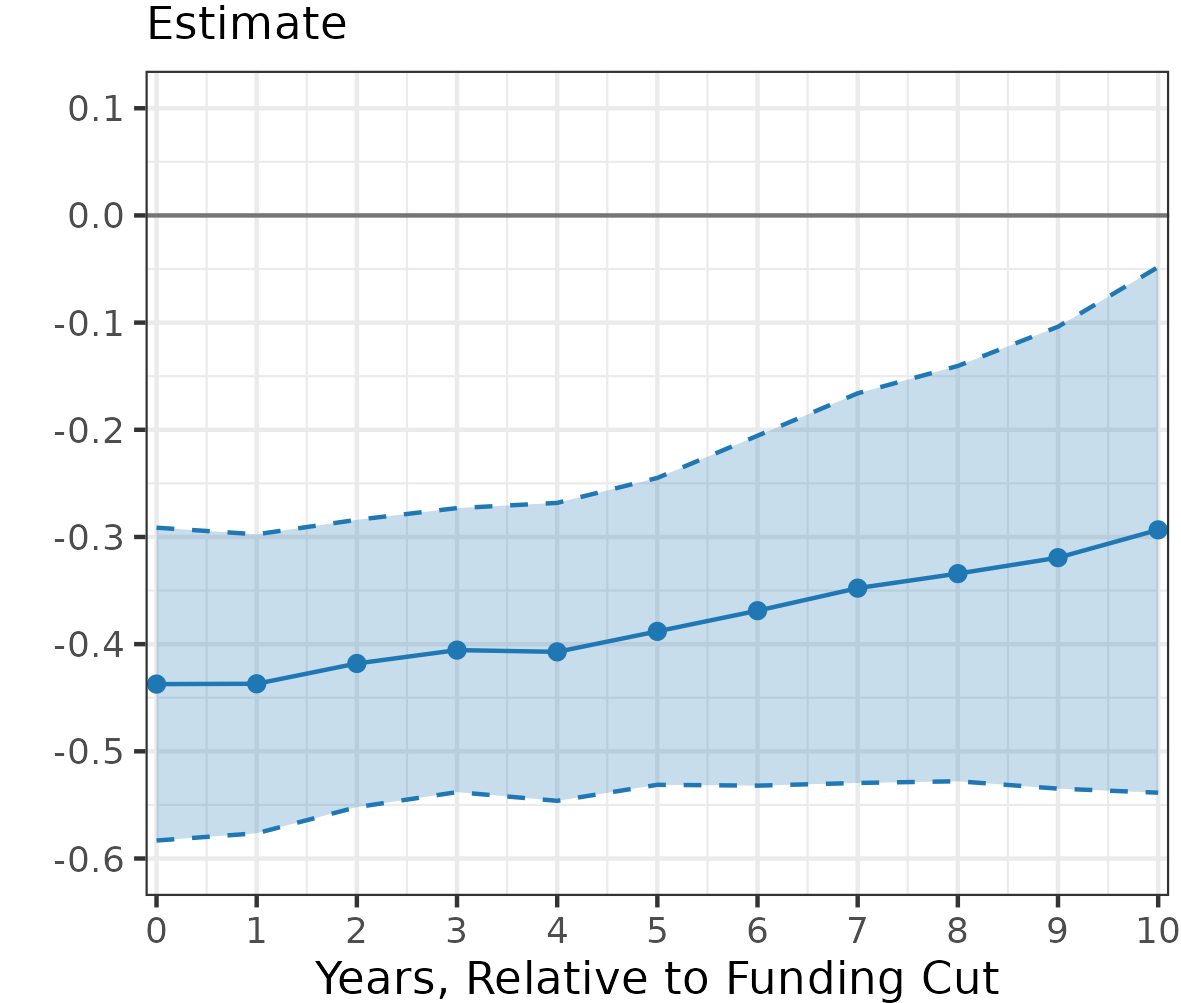
\includegraphics[width=\textwidth]{figures/lecturer-count-lp.png}
        \label{fig:lecturer-count-lp}
    \end{subfigure}
    \begin{subfigure}[b]{0.495\textwidth}
        \centering
        \caption{Assistant Professors.}
        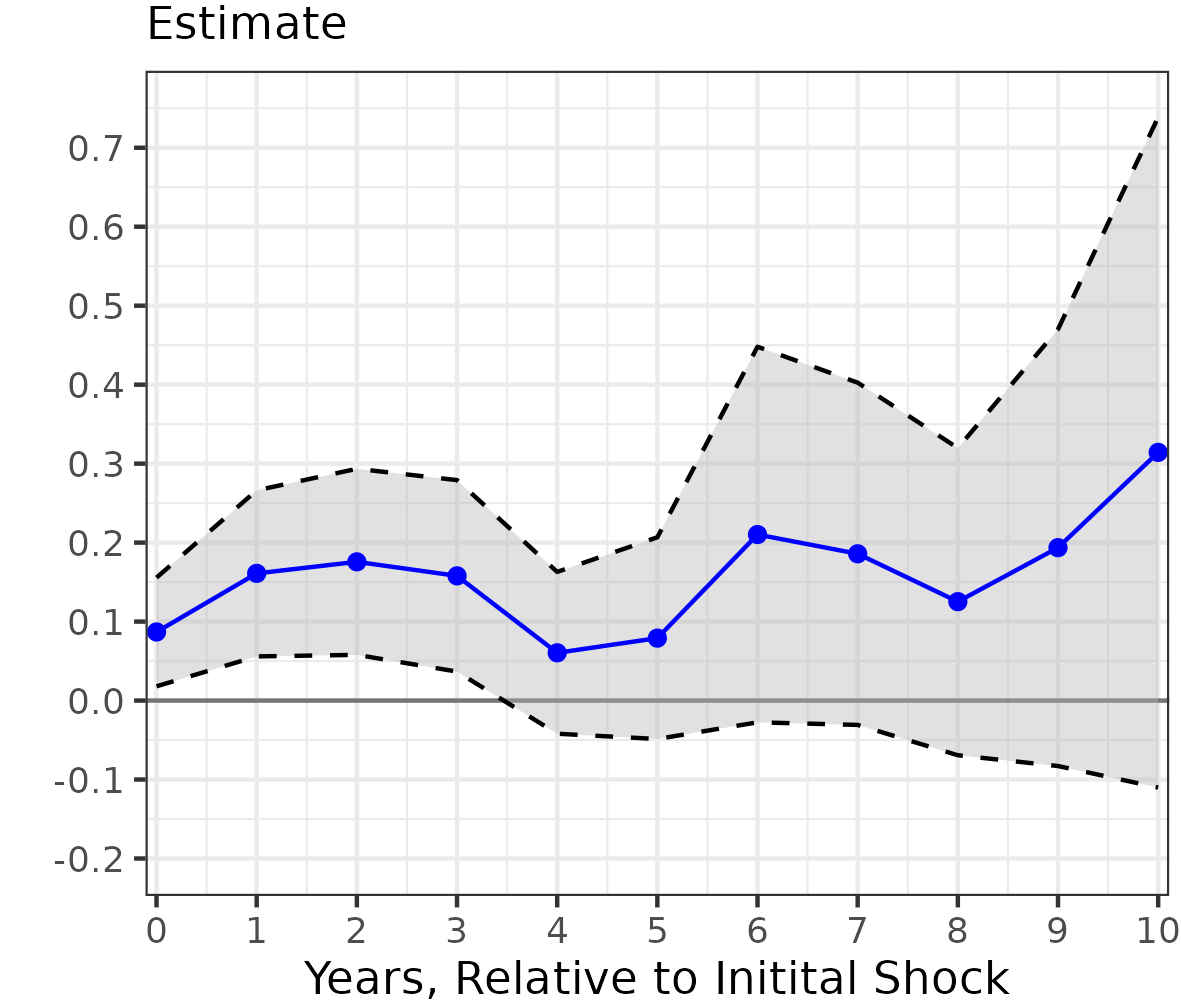
\includegraphics[width=\textwidth]{figures/assistant-count-lp.png}
        \label{fig:assistant-count-lp}
    \end{subfigure}
    \begin{subfigure}[b]{0.495\textwidth}
        \centering
        \caption{Full Professors.}
        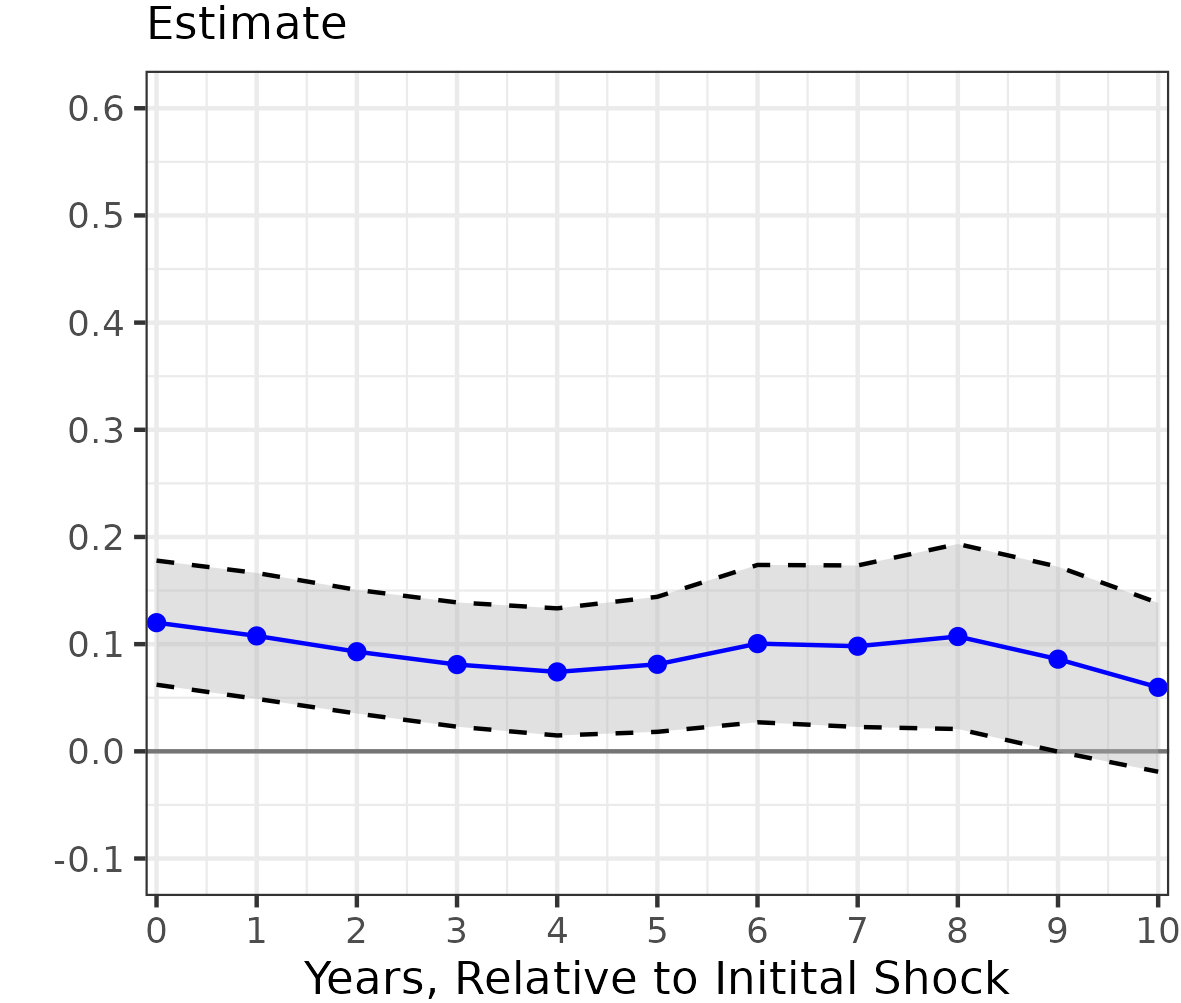
\includegraphics[width=\textwidth]{figures/full-count-lp.png}
        \label{fig:full-count-lp}
    \end{subfigure}
    \begin{subfigure}[b]{0.495\textwidth}
        \centering
        \caption{All Professors.}
        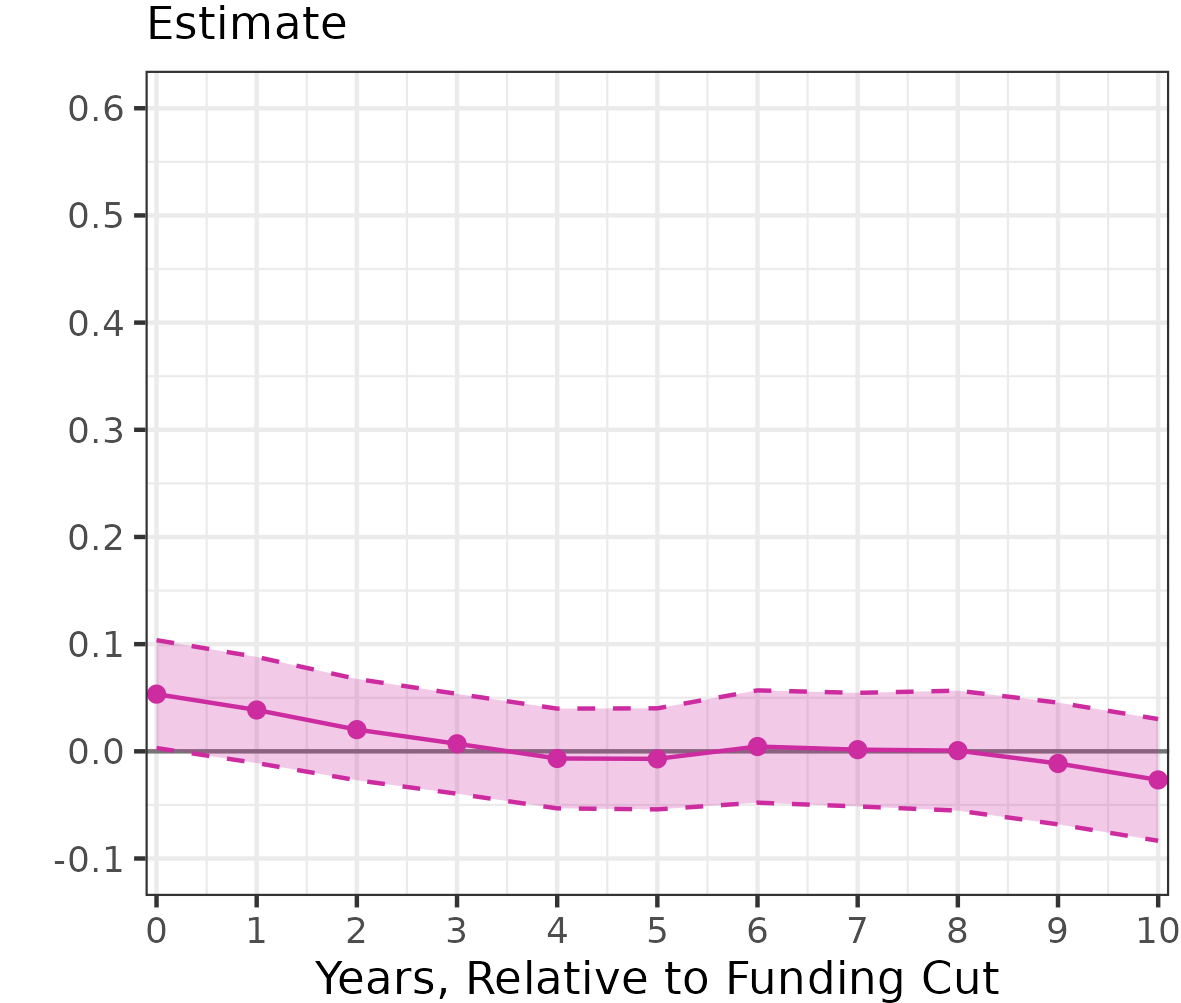
\includegraphics[width=\textwidth]{figures/all-count-lp.png}
        \label{fig:all-count-lp}
    \end{subfigure}
    \label{fig:count-lp}
\end{figure}

Decreases in university revenues (via state funding shocks) affect faculty composition for at most 4 years after the initial revenue shock.
A 10\% decrease in state funding increases count of lecturers per student by 4\% for the first two years after the initial shock.
While count of assistant professors decreases 10 to 18.5\% three years later;
count of tenured professors decreases 9 to 6\% three years later.
Together, the total count of professors per student decreases around 1\% for three years after the initial funding shock, and the effect is not distinguishable from zero four years after.

\autoref{fig:count-lp} represents these estimates, using the local projection method, as a series of impulse responses for each outcome of professor count.
The mechanism that explains the changes in faculty composition are, however, not clear at this unit of analysis; individual data are needed to delve deeper.

\subsection{Individual Professor Outcomes}

I first examine whether a shock to the university's revenues affects the salaries of professors at the university.
The first outcome is first-year salary for each professor by their position;
\autoref{tab:newhiresalaries-shock-illinois-rolling} presents 2SLS estimates for the elasticity of total salaries with respect to university revenues, among the sample with a year of starting employment after 2010.
New hires of assistant, full, or administrative position professors are not related to revenues, via a shock to appropriations in their first-year of employment.
Yet, the starting salary of lecturers is 3.8\% higher given an increase in their hiring university's state funding of 10\%.

\begin{table}[h!]
    \singlespacing
    \centering
    \caption{2SLS Estimates for Faculty Salaries, in First-Year, at Illinois Universities.}
    \makebox[\textwidth][c]{
\begin{tabular}{@{\extracolsep{5pt}}lccccc} 
\\[-1.8ex]\hline 
\hline \\[-1.8ex] 
 & \multicolumn{5}{c}{Dependent Variable: Salaries by Professor Group} \\ 
\cline{2-6} 
 & Lecturer & Assistant & Full & Admin & All \\ 
\\[-1.8ex] & (1) & (2) & (3) & (4) & (5)\\ 
\hline \\[-1.8ex] 
 State Funding & 0.057 & $-$0.123 & $-$0.051 & $-$0.039 & $-$0.016 \\ 
  & (0.073) & (0.034) & (0.083) & (0.048) & (0.059) \\ 
 \hline \\[-1.8ex] 
Observations & 8,985 & 5,133 & 1,265 & 3,175 & 18,558 \\ 
R$^{2}$ & 0.297 & 0.061 & 0.043 & 0.240 & 0.220 \\ 
\hline 
\hline \\[-1.8ex] 
\end{tabular} 
}
    \begin{flushleft}
        \footnotesize
        \textbf{Note}: Standard errors are clustered at the institution and first year of employment level. 
    \end{flushleft}
    \label{tab:newhiresalaries-shock-illinois-rolling}
\end{table}

Regarding total salary for every year of employment, \autoref{tab:facultysalaries-shock-illinois-rolling} presents estimates for the elasticity of total salary with respect to university revenues, for the entire sample of professors hired after 2010.\footnote{
    Recall that this is a subsample of the entire data, that the rolling shift-share instrument is only defined for the sample with an observed hiring date in the years 2011-2021.
}
The elasticity is non-distinguishable from zero among any position, implying that long-term salaries are not related to state funding.
\autoref{tab:facultysalaries-shock-illinois} presents the same model, for the sample of all professors and using the instrument based in years 1990-1993, similarly finding no relationship.

\begin{table}[h!]
    \singlespacing
    \centering
    \caption{2SLS Estimates for Faculty Salaries at Illinois Universities.}
    \makebox[\textwidth][c]{
\begin{tabular}{@{\extracolsep{5pt}}lccccc} 
\\[-1.8ex]\hline 
\hline \\[-1.8ex] 
 & \multicolumn{5}{c}{Dependent Variable: Annual Salaries} \\ 
\cline{2-6} 
 & Lecturer & Assistant & Full & Admin & All \\ 
\\[-1.8ex] & (1) & (2) & (3) & (4) & (5)\\ 
\hline \\[-1.8ex] 
 State Funding & 0.007 & $-$0.072 & $-$0.043 & $-$0.010 & $-$0.012 \\ 
  & (0.095) & (0.041) & (0.038) & (0.049) & (0.086) \\ 
 \hline \\[-1.8ex] 
Observations & 26,324 & 22,328 & 9,065 & 11,529 & 69,246 \\ 
R$^{2}$ & 0.220 & 0.051 & 0.069 & 0.144 & 0.163 \\ 
\hline 
\hline \\[-1.8ex] 
\end{tabular} 
}
    \begin{flushleft}
        \footnotesize
        \textbf{Note}: Standard errors are clustered at the institution-year level.
    \end{flushleft}
    \label{tab:facultysalaries-shock-illinois-rolling}
\end{table}

Note that professor position (assistant, associate, full) is also an outcome, thanks to the promotion channel: a university may be less able to promote their professors to higher paying positions when their revenues are constrained.
\autoref{tab:promotion-shock-illinois-rolling} shows estimates where the outcome is rate of promotion within each professor position.
The lecturer position describes the sample of professors who were ever listed as a non-tenure track lecturer and the binary for promotion equals one in a year they achieved an assistant professor position; assistant the same for the assistant to associate professor promotion; associate same for associate to full promotion.
There is no discernible relationship between revenues and promotion among any position.\footnote{
    \autoref{tab:promotion-shock-illinois} shows estimates using the base-year instrument among the entire sample, finding the same results.
}
Furthermore, local projection estimates (\autoref{fig:promoted-illinois-lp}) show that the there is no promotion effect, among all professors, for any of the following years either.
Lastly, \autoref{tab:facultyleaving-shock-illinois-rolling}, \ref{tab:facultyleaving-shock-illinois} describes estimates for rate of exit from the employing university among Illinois professors, and finds no relationship with university revenues.
